\documentclass[12pt, a4paper]{article}
\usepackage[utf8]{inputenc}
\usepackage{amssymb}
\usepackage{indentfirst}
\usepackage{listings}
\usepackage{enumitem}
\usepackage{comment}
\usepackage{graphicx}
\usepackage{color}
\usepackage[portuguese]{babel}
\usepackage{geometry}
\geometry{legalpaper, a4paper,
 total={170mm,257mm},
 left=20mm,
 top=20mm}
\setlength{\voffset}{-10mm}
\definecolor{dkgreen}{rgb}{0,0.6,0}
\definecolor{gray}{rgb}{0.5,0.5,0.5}
\definecolor{mauve}{rgb}{0.58,0,0.82}

\lstset{frame=tb,
  language=Java,
  aboveskip=3mm,
  belowskip=3mm,
  showstringspaces=false,
  columns=flexible,
  basicstyle={\small\ttfamily},
  numbers=none,
  numberstyle=\tiny\color{gray},
  keywordstyle=\color{blue},
  commentstyle=\color{dkgreen},
  stringstyle=\color{mauve},
  breaklines=true,
  breakatwhitespace=true,
  tabsize=3
}

\newcommand{\tit}[1]{\textit{#1}}
\newcommand{\tb}[1]{\textbf{#1}}
\newcommand{\tbi}[1]{\textbf{\textit{#1}}}

\newcommand{\bitem}[2]{ \tb{(\tit{#1}) {#2}}}
\newcommand{\iitem}[1]{(\tit{#1})}

\newcommand{\oo}{orientação à objetos}
\newcommand{\sw}{\tit{software}}
\newcommand{\ssw}{\tit{software} }

\newcommand{\question}[1]{\item \tb{#1}}
\newcommand{\answer}[1]{\par #1}

\newcommand{\quotes}[1]{``#1''}

\title{Módulo 2 - Atividade Individual \\
  \large Processo de Desenvolvimento de Software}

\author{Wellington Espindula}
\date{Janeiro de 2020}

\begin{document}
    \maketitle
    
    \begin{enumerate}[label=\textbf{\arabic*.}]
        \question{Defina modelo de processo de software. Escolha dois dos modelos de processo de software existentes, descreva-os, discuta suas vantagens e desvantagens de forma comparativa.}
        \answer{
        Dada a existência de diferentes processos de desenvolvimento de \sw, os modelos de \ssw são uma forma de \tb{agrupar os processos de desenvolvimento de forma a criar uma \quotes{família de processos}} de desenvolvimento de \sw. Dessa forma, modelos de processo de \ssw são modelos criados com o intuito de representar de forma simples um processo de \ssw e abstrair as características importantes de processos específicos. Dois exemplos de modelos de processo de \ssw são:
        \begin{itemize}
            \item \tb{Modelo em Cascata (\tit{Waterfall}):} Um dos primeiros modelos utilizados no desenvolvimento de \sw, o modelo em cascata consiste em um processo de \tb{desenvolvimento linear subdividido em fases}. Isto é, cada fase do projeto é realizada seguindo uma ordem. Inicialmente, realiza-se o levantamento dos requisitos. Só após esta fase estar completa, pode-se realizar o projeto do sistema, e assim consecutivamente. Por consequência, o \tb{planejamento deve ser cauteloso}, visto que o modelo de desenvolvimento oferece \tb{baixa flexibilidade à mudanças}.
            \item \tb{Modelo Evolucionário (Prototipação):} \tb{Rápido e barato}, o modelo evolucional envolve a \tb{prototipação}. A prototipação serve para testar ideias, viabilidade, demonstrar conceitos, etc. Dessa forma, a prototipação não necessariamente precisa de uma implementação visto que o \tb{protótipo pode vir a ser descartado} e substituído por uma nova implementação de um sistema final.

        \end{itemize}
        
        Em relação à riscos e ao custo do erro, o modelo evolucionário se torna melhor, dado que o protótipo é rápido e barato e permite vislumbrar a viabilidade do produto. Já o modelo cascata necessidade de fases muito bem definidas e inflexíveis, então se houver erro, em fase de definição de requisitos por exemplo, ou o projeto for inviável será muito custoso, porque isso só será notado em fases mais avançadas do projeto - necessitando voltar às fases iniciais ou arruinando um projeto que já houve alto custo envolvido em diversas fases.\\
        Ambos os projetos envolvem uma boa compreensão dos requisitos. Enquanto o evolucional pode utilizar o protótipo para discutir modelos, ideias e chegar em uma maior compreensão dos requisitos do usuário, o método em cascata necessita de uma alta compreensão dos requisitos do sistema em fase inicial e estes se mantêm estáveis. \\
        O modelo em cascata permite pouca participação do usuário e torna o projeto rígido à mudanças. Em contrapartida, o modelo evolucionário pode apresentar grande participação do usuário mas, ao mesmo tempo, pode apresentar mais variações nos requisitos ao passo que novos requisitos podem surgir a cada nova versão do protótipo avaliado pelo usuário. \\
        Um grande problema do uso do modelo evolucional é que existe uma grande dificuldade em convencer o usuário da necessidade do descarte do protótipo. Bem como o processo evolucional torna o processo do \ssw pouco visível, visto que o progresso é mensurado pelos artefatos produzidos e outras preocupações mais abrangentes de \ssw (como documentação e testes) podem ficar em segundo plano.
        } \\
        
        \question{Descreva, com suas palavras, as principais atividades do processo de desenvolvimento de software e respectivos documentos gerados em cada atividade.}
        \answer{
            \begin{itemize}
                \item \tb{Especificação:} Atividade cujo objetivo é entender qual produto será criado, se é possível, quais são as restrições do produto, o que é essencial para este, quais são seus requisitos e como será realizado. Dessa forma a especificação é composta de atividades como estudo de viabilidade, análise, especificação e validação de requisitos. O maior documento gerado é a documentação da especificação de requisitos, que deve informar os requisitos de negócio, bem como requisitos de sistema. Ademais, a fase de Análise de requisitos também pode envolver protótipos, provas de conceito e modelos de sistema.
                \item \tb{Projeto e Implementação:} Tornar a especificação em um sistema de \sw. Dessa forma, essa atividade envolve tornar as especificações em um projeto de \ssw e implementá-lo. Dentre as etapas de projetos, tem-se o projeto de arquitetura, os projetos de componentes e o projeto de banco de dados. A programação envolve implementar o projeto em uma (ou mais) linguagem de programação. Na implementação, faz-se de extrema importância os testes e depuração.
                \item \tb{Verificação e Validação:} As atividades de verificação e validação servem para verificar se o sistema está em conformidade com o que foi especificado e validar o \ssw a partir do ponto de vista do cliente. Portanto, essa etapa envolve os testes de desenvolvimento, de integração e sistema e testes de aceitação. 
                \item \tb{Evolução:} Etapa responsável por evoluir o sistema envolvendo  manutenção, correção de \tit{bugs} e desenvolvimento de novas funcionalidades. Como o \sw, diferentemente de outros produtos, é flexível, essa etapa é de extrema importância porque surgem novas demandas e o \ssw tem de se adaptar a isso. Ademais, é necessário detectar e corrigir os problemas existentes com a finalidade de diminuir a \quotes{deterioração} do sistema.
            \end{itemize}
        }
        
        \question{Modelo em Cascata. Em que tipos de projeto se poderia utilizar o modelo cascata?}
        \answer{
        O modelo em cascata consiste em um processo de desenvolvimento linear subdividido em fases. O modelo em cascata é \tb{muito utilizado em projetos de grande porte que são desenvolvidos em lugares diversos.} Esse modelo é muito recomendado para projetos grandes com \tb{requisitos bem definidos e pouco voláteis.}
        }
        \\
        
        \question{Modelo Incremental. Descreva um exemplo de projeto de software suscetível ao uso de desenvolvimento incremental. Descreva as etapas de cada incremento.}
        \answer{
            O Modelo Incremental organiza as atividades em incrementos, aperfeiçoando o \ssw paulatinamente. Um exemplo possível seria a de uma loja on-line, que tem-se uma ideia inicial de como deve ser mas que deve ser melhorada ao longo do tempo com novos requisitos do usuário. As iterações poderiam ser \iitem{i} Desenvolver página inicial (estática) com produtos e preços; \iitem{ii} Desenvolver um CRUD de produtos; \iitem{iii} Interligar o página de produtos com os produtos cadastrados; \iitem{iii} Criar página de administrador com autenticação simples; \iitem{iv} Interligar página de administrador com CRUD de produtos; \iitem{v} Criar uma página de carrinho de compras; \iitem{vi} Criar um CRUD de pedidos; \iitem{vii} Integrar carrinho de compras com pedidos e com um \ssw de pagamento on-line; \iitem{viii} Integrar pedidos de compras com página de administrador; ...
        }
        \\
        
        \question{Considere o seguinte cenário. Você faz parte da equipe de um projeto de software e deve escolher um modelo de processo de desenvolvimento de software a ser seguido neste projeto. O software a ser desenvolvido visa auxiliar no gerenciamento de um hospital público, e tem as seguintes características.
            \begin{enumerate}[label=\textbf{\arabic*.}]
                \item O projeto consiste na criação de um software para dar suporte ao (a) agendamento de consultas; (b) realização de consultas; (c) cadastro de pacientes; e (d) verificação do seguimento, pelos médicos e enfermeiras, de protocolos estabelecidos pelo governo.
                \item Nem o órgão do governo que solicitou o projeto, nem seus (perspectivos) usuários sabem exatamente todas as funcionalidades que o sistema deve oferecer.
                \item O software deve entrar em produção o mais rápido possível.
            \end{enumerate} 
        Qual o modelo de processo de desenvolvimento de software que você escolheria para este projeto? Explique sua resposta, justificando-a com base no cenário acima descrito.}
        \answer{
            Para esse projeto utilizaria o Modelo Iterativo Incremental. Poderia, inclusive, ser utilizado metodologias ágeis para o desenvolvimento do \ssw em questão. Visto que as funcionalidades mais básicas do \ssw estão especificadas no item 1, poderia-se construir um sistema de forma ágil utilizando \tit{Extreme Programming} (XP) por exemplo. Dessa forma, a primeira \tit{release} entraria em produção o mais rápido possível com as funcionalidades mais básicas de acordo com os itens 1 e 3. Como o item 2 afirma que os usuários ainda não sabem exatamente todos as funcionalidades e requisitos, o modelo iterativo incremental usando metodologias ágeis ampliaria a participação dos usuários e tornaria o processo de aperfeiçoamento do \ssw contínuo, assim os usuários poderão ao longo do processo de desenvolvimento ter cada vez mais claro o que desejam no \sw. Desse modo, o \ssw teria \tit{releases} mais frequentes envolvendo novas funcionalidades, \tit{features} e correção de \tit{bugs}.
            }
        \\
        
        \question{Marque verdadeiro (V) ou falso (F). Os métodos ágeis...} \\
        (\tb{V}) ... são um suplemento aos métodos existentes, e não uma metodologia completa. \\
        (\tb{F}) ... são um processo prescritivo que detalha os passos que devem ser feitos para o desenvolvimento de um sistema de software. \\
        (\tb{V}) ... são uma forma efetiva de se trabalhar em conjunto para atingir as necessidades das partes interessadas no projeto. \\
        (\tb{V}) ... focam em simplicidade, sempre trabalhando para eliminar a complexidade do sistema. \\
        (\tb{V}) ... têm como princípios a satisfação dos clientes, a estabilização de requisitos, e entregas de software operacional frequentemente. \\
        (\tb{V}) ... funcionam na prática, não sendo teoria acadêmica. \\
        (\tb{V}) ... são para o desenvolvedor médio, mas não são um substituto de pessoas competentes. \\
        (\tb{F}) ... atacam a documentação dos sistemas de software, visto que eles aumentam significantemente o
tempo e custo de desenvolvimento de software. \\
        (\tb{V}) ... têm como dificuldade o envolvimento do cliente no desenvolvimento de software e que seja capaz de passar o tempo com a equipe de desenvolvimento. \\
        (\tb{F}) ... pregam o não uso de ferramentas CASE, já que os documentos produzidos nelas são raramente utilizados e usualmente ficam desatualizados. \\
    
        \question{Escolha duas afirmações das apresentadas acima que você considera como falsas e explique o motivo, indicando o que deveria ser modificado para que elas se tornem verdadeiras.}
        \answer{
        \begin{itemize}
            \item \tb{Os métodos ágeis são um processo prescritivo que detalha os passos que devem ser feitos para o desenvolvimento de um sistema de software}: Os métodos ágeis são métodos mais adaptativos que prescritivos, dito isso, eles não criam uma documentação muito detalhada sobre o desenvolvimento de um sistema já que focam em se adaptar às mudanças de especificações e demandas. 
            \item \tb{Os métodos ágeis pregam o não uso de ferramentas CASE, já que os documentos produzidos nelas são raramente utilizados e usualmente ficam desatualizados.}: Por mais que os métodos ágeis foquem mais em um \ssw funcional que em outros aspectos de \ssw - como uma documentação detalhada -, estes não atacam as ferramentas CASE, mas, sim, envolvem a atenção contínua à excelência técnica. Então, testes, refatoração, uso de \tit{Design Patterns} fazem parte do desenvolvimento ágil.
        \end{itemize}
        }
        
        \newpage
        \question{Com relação ao Rational Unified Process (RUP), responda as questões abaixo.}
        \begin{figure}[!ht]
            \centering
            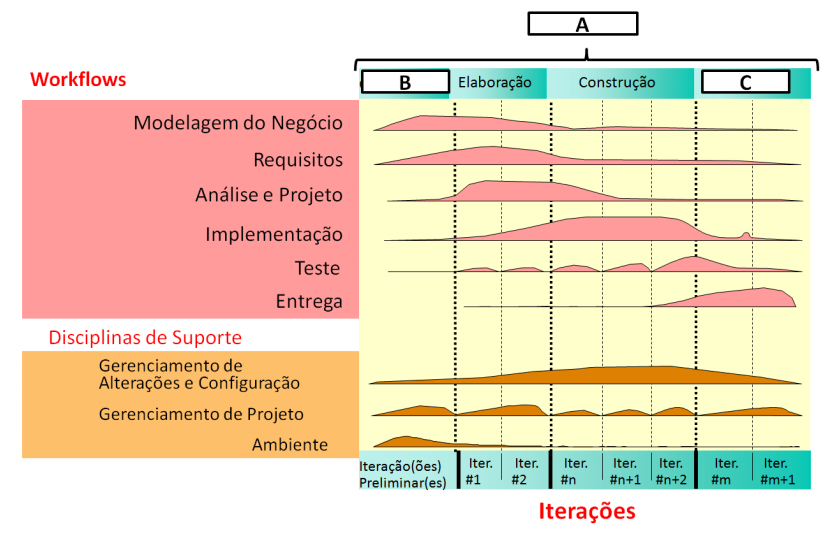
\includegraphics[width=0.75\textwidth,keepaspectratio]{rup}
            \label{fig:my_label}
        \end{figure}
        \par Considerando o diagrama do RUP acima, diga qual termo completaria cada um dos campos em branco no diagrama.
        \\
        \begin{itemize}
            \item \tb{Campo A:} Fases
            \item \tb{Campo B:} Concepção
            \item \tb{Campo C:} Transição
        \end{itemize}
    \end{enumerate}



    
\end{document}